\documentclass[border=4pt]{standalone}
\usepackage{amsmath,amssymb}
\usepackage[scaled=0.92]{helvet}
\renewcommand{\familydefault}{\sfdefault}
\usepackage{tikz}
\usetikzlibrary{positioning,arrows.meta,fit,calc}
\definecolor{cInD}{HTML}{3B6EA8}
\definecolor{cGD}{HTML}{C76E00}
\definecolor{cTD}{HTML}{2E7D32}
\definecolor{cOD}{HTML}{7B3F99}
\definecolor{cRD}{HTML}{B23A3A}
\definecolor{cGy}{HTML}{6B6B6B}
\tikzset{
  box/.style={draw=#1!80!black, fill=#1!10, rounded corners=3pt, align=center, font=\small, inner sep=4pt, line width=0.6pt},
  arr/.style={-{Stealth[length=2.2mm]}, line width=0.8pt, draw=black!70},
  lbl/.style={font=\footnotesize, text=black!75, align=center},
  seg/.style={draw=white, line width=0.8pt, fill=#1, minimum height=7mm, font=\footnotesize, text=white, align=center, inner sep=1pt},
}
\begin{document}
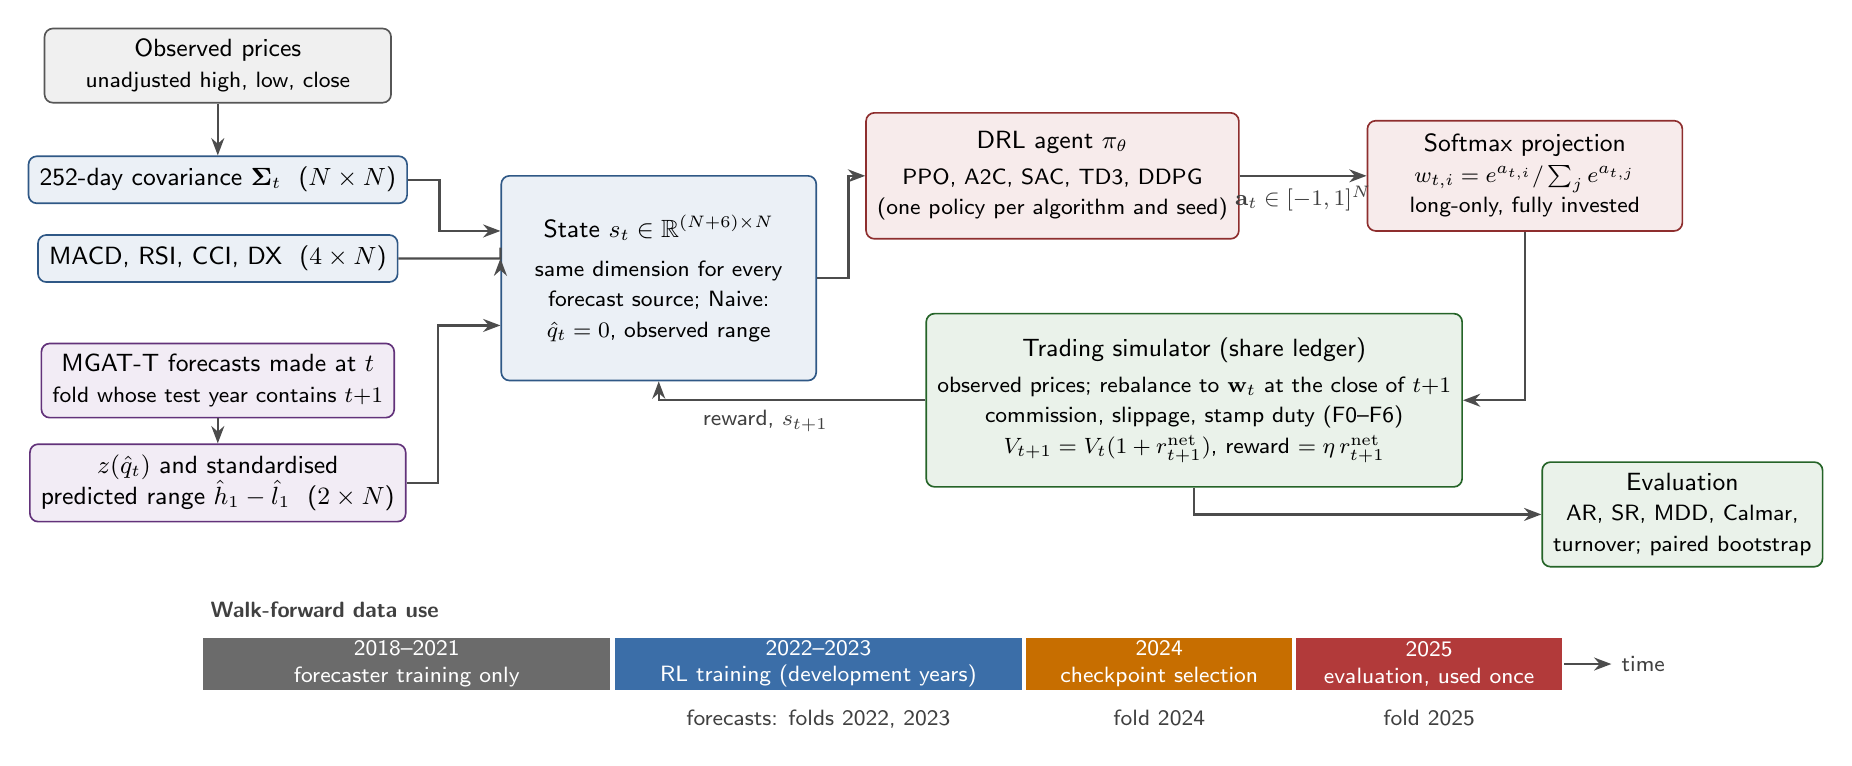
\begin{tikzpicture}
% inputs
\node[box=cGy, minimum width=44mm] (px) at (0,0) {Observed prices\\ {\footnotesize unadjusted high, low, close}};
\node[box=cInD, minimum width=44mm] (cov) at (0,-1.45) {252-day covariance $\boldsymbol{\Sigma}_t$ \ ($N\times N$)};
\node[box=cInD, minimum width=44mm] (tech) at (0,-2.45) {MACD, RSI, CCI, DX \ ($4\times N$)};
\node[box=cOD, minimum width=44mm] (fc) at (0,-4.0) {MGAT-T forecasts made at $t$\\ {\footnotesize fold whose test year contains $t{+}1$}};
\node[box=cOD, minimum width=44mm] (frow) at (0,-5.3) {$z(\hat q_t)$ and standardised\\ predicted range $\hat h_1-\hat l_1$ \ ($2\times N$)};
\draw[arr] (px)--(cov); \draw[arr] (fc)--(frow);
% state
\node[box=cInD, minimum width=40mm, minimum height=26mm] (state) at (5.6,-2.7) {State $s_t\in\mathbb{R}^{(N+6)\times N}$\\[3pt] {\footnotesize same dimension for every}\\ {\footnotesize forecast source; Naive:}\\ {\footnotesize $\hat q_t=0$, observed range}};
\draw[arr] (cov.east) -- ++(4mm,0) |- ($(state.west)+(0,6mm)$);
\draw[arr] (tech.east) -- ($(state.west)+(0,0.25)$ -| tech.east) -- ($(state.west)+(0,0.25)$);
\draw[arr] (frow.east) -- ++(4mm,0) |- ($(state.west)+(0,-6mm)$);
% agent and projection
\node[box=cRD, minimum width=40mm, minimum height=16mm] (agent) at (10.6,-1.4) {DRL agent $\pi_\theta$\\[2pt] {\footnotesize PPO, A2C, SAC, TD3, DDPG}\\ {\footnotesize (one policy per algorithm and seed)}};
\node[box=cRD, minimum width=40mm, minimum height=14mm] (proj) at (16.6,-1.4) {Softmax projection\\ {\footnotesize $w_{t,i}=e^{a_{t,i}}/\sum_j e^{a_{t,j}}$}\\ {\footnotesize long-only, fully invested}};
\draw[arr] (state.east) -- ++(4mm,0) |- (agent.west);
\draw[arr] (agent)--node[lbl, below]{$\mathbf{a}_t\in[-1,1]^N$}(proj);
% simulator
\node[box=cTD, minimum width=56mm, minimum height=22mm] (sim) at (12.4,-4.25) {Trading simulator (share ledger)\\[2pt]
  {\footnotesize observed prices; rebalance to $\mathbf{w}_t$ at the close of $t{+}1$}\\ {\footnotesize commission, slippage, stamp duty (F0--F6)}\\
  {\footnotesize $V_{t+1}=V_t(1+r^{\mathrm{net}}_{t+1})$, reward $=\eta\,r^{\mathrm{net}}_{t+1}$}};
\draw[arr] (proj.south) |- (sim.east);
\draw[arr] (sim.west) -| node[lbl, below, pos=0.3]{reward, $s_{t+1}$} (state.south);
\node[box=cTD, minimum width=34mm] (met) at (18.6,-5.7) {Evaluation\\ {\footnotesize AR, SR, MDD, Calmar,}\\ {\footnotesize turnover; paired bootstrap}};
\draw[arr] (sim.south) |- (met.west);
% timeline
\def\y{-7.6}
\node[seg=cGy, minimum width=52mm] (s1) at (2.4,\y) {2018--2021\\ forecaster training only};
\node[seg=cInD, minimum width=52mm, right=0pt of s1] (s2) {2022--2023\\ RL training (development years)};
\node[seg=cGD, minimum width=34mm, right=0pt of s2] (s3) {2024\\ checkpoint selection};
\node[seg=cRD, minimum width=34mm, right=0pt of s3] (s4) {2025\\ evaluation, used once};
\draw[arr] (s4.east) -- ++(6mm,0) node[lbl, right]{time};
\node[lbl, below=1mm of s2] {forecasts: folds 2022, 2023};
\node[lbl, below=1mm of s3] {fold 2024};
\node[lbl, below=1mm of s4] {fold 2025};
\node[lbl, above=1mm of s1.north west, anchor=south west] {\textbf{Walk-forward data use}};
\end{tikzpicture}
\end{document}
